\documentclass[12pt,oneside]{book}
\usepackage{listings}
\usepackage{amsmath,amssymb,graphicx,float}
\usepackage[cm]{fullpage}
\usepackage[inline]{enumitem}
\usepackage{xcolor,xparse,realboxes}
\usepackage{lmodern}
\usepackage{hyperref}
\hypersetup{
    colorlinks,
    citecolor=black,
    filecolor=black,
    linkcolor=blue,
    urlcolor=grey
}
\newcommand{\abs}[1]{\left\vert#1\right\vert}
\newcommand{\xn}[2]{{#1}_1{#2}{#1}_2{#2}\dots{#2}{#1}_n}
\newcommand*\lstinputpath[1]{\lstset{language=[90]Fortran,captionpos=b,numbers=left,showstringspaces=false,
keywordstyle=\color{blue},
commentstyle=\color{green},
morecomment=[l]{!\ },inputpath=#1}}

\lstinputpath{code}
\newcommand{\code}[1]{\lstinline[keywordstyle=\color{black},basicstyle=\ttfamily]{#1}}
\begin{document}
    \title{Fortran}
    \author{Mehedi hasan}
    \maketitle
    \newpage
    \section*{Preface}
    This is a compilation of lecture notes with some books and my own thoughts. This document is not a holy text. So, if there is a mistake, solve it by your own judgement.
    \pagenumbering{roman}
    \newpage
    \tableofcontents
    \newpage
    \lstlistoflistings
    \newpage
    \pagenumbering{arabic}
    \part{Notes}
    \chapter{Introduction}
    \section{History}
    Fortran (FORmula TRANslation) was the first high-level programming language.
    It was devised by John Backus in 1953. 
    The first Fortran compiler was produced in 1957. 
    Fortran is highly standardized making it extremely portable (able to run on a wide range of platforms).
    It has passed through a sequence of international standards those underlined below being the most important.
    \begin{itemize}
        \item Fortran 66 - original ANSI standard (accepted 1972)
        \item Fortran 77 - ANSI x3.9-1978 - standard programming
        \item Fortran 95 - ISO/IEC 1539-1 1997 (minor revision)
        \item Fortran 2003 - ISO/IEC 1539-1 : 2004 (E) object oriented programming interpretability with C
        \item Fortran 2008 - ISO/IEC 1539-1 : 2010 - Co array (parallel programming)
        \item Fortran 2018 - Imminent !
    \end{itemize}
    Fortran is widely used in high performance computing (HPC). Where its ability to run code in parallel on a large number of process makes it popular for computationability demanding tasks a science and engineering.
    \section{Source Code and Executable Code}
    In all high-level languages (Fortran, C++, Java, Python, \dots ) programmes are written in source code.

    This is a human readable set of instructions that can be created or modified on any computer with any text editor. File types identifies the programming language. eg. Fortran file has file types .f90 or .f95.
    \section{Compiler}
    The job of compiler is to turn source code into machine readable executable code under windows, executable files have file type .exe.\\

    Producing executable code is actually a two-stage process.
    \begin{itemize}
        \item compiling converts each individual source file into object code.
        \item object code linking combines all the object files with additional library routine to create an executable program.
    \end{itemize}
    \section{Fortran Compiler}
    \begin{enumerate}
        \item nagfor
        \item IFORT (Intel Fortran Compiler)
        \item GNU Fortran (gfortran)
        \item Silverfrost FTN95
    \end{enumerate}
    \section{Creating and Compiling Fortran Code}
    You may create, edit, compile and run a Fortran program either 
    \begin{itemize}
        \item From a command line
        \item in an Integrated Development Environment (IDE)
    \end{itemize}
    You can create Fortran source code with any text editor. eg. Notepad.
    \section{Some Example Code}
    \subsection{Hello World}
    \lstinputlisting[caption= Hello world in Fortran]{hello.f90}
    \subsection{Quadratic Equation Solve}
    The well-known solutions of the quadratic equation $ Ax^2+Bx+C=0 $ are $ x=\frac{\displaystyle-B\pm\sqrt{ B^2-4AC}}{\displaystyle 2A} $
    The program might look like the following:
    \lstinputlisting[caption=Quadratic Solver]{quadratic.f90}
    \chapter{Basic Elements of Fortran}
    \section{Variable Names}
    A name is a symbolic link to a location in memory. A variable is a memory location whose value may be changed during execution.
    Names must:
    \begin{itemize}
        \item have between 1 and 63 alphanumeric character (alphabet, digits and underscore).
        \item start with a letter.
    \end{itemize}
    One should not use Fortran keyword or standard intrinsic (in-built) function as a variable name.
    Tempting names that should be avoided in this respect include: counts, len, product, range, scale, size, sum, tiny.
    The following are valid variable names: \code{SUST_UNITED}, \code{as_easy_as_123}.
    The following are not: \code{Math+Physics} ('+' is not allowed), \code{999help} (starts with a number), \code{Hello!} ('!' would be treated a comment not as a part of the variable name)
    \section{Data Types}
    In Fortran there are 5 intrinsic data types.
    \begin{enumerate}
        \item Integer
        \item Real 
        \item Complex
        \item Character
        \item Logical
    \end{enumerate}
    The first three are numeric types while the other two are non-numeric types. 
    It is also possible to have derived data types and pointers.
    \subsection{Integer}
    Integer constants are whole numbers without a decimal point. e.g. 100, +16, -14, 0, 666. They are stored exactly, but their range is limited; typically $ -2^{n-1} $ to $ 2^{n-1}-1 $. Where $ n $ is either $ 16 $ (for 2-byte integer) or 32 (for 4-byte integer). 
    It is possible to change the default range using the \code{kind} type parameter.
    \subsection{Real}
    Real constant has a decimal point and maybe entered as either fixed point, eg. 442.2 or floating point, eg. 4.122e+02.
    Real constants are stored in exponential form in memory, no matter how they are entered. 
    They are accurate only to a finite machine precision (which again, can be changed using the \code{kind} type parameter).
    \subsection{Complex}
    Complex constants consist of paired real number corresponding to real and imaginary parts. eg. (2.0, 3.0) corresponds to $ 2+3i $.
    \subsection{Character}
    Character constants consists of strings of characters enclosed by a pair of delimiters, which may be either single (') or double (") quotes. eg. \code{"This is a string", 'Department of Mathematics'}. The delimiter themselves are not part of the string.
    \subsection{Logical}
    Logical constants may be either true or false.
    \section{A program to compute square root of a number}
    \[x_{n+1}=\frac{1}{2}\left(x_n+\frac{a}{x_n}\right)\to \sqrt{a}\]
    Using \code{if (...) exit}
    \lstinputlisting[caption=Newton's method for finding square root (using if)]{rootNewtonIf.f90}
    Using \code{do while}
    \lstinputlisting[caption=Newton's method for finding square root (using do while)]{rootNewtonDoWhile.f90}
    \section{Declaration of Variable}
    \subsection{Type}
    Variables should be declared (that is, have either data types defined and memory set aside for them) before any executable statements. This is achieved by a type declaration statement of form, eg. \begin{lstlisting}[numbers=none]
        integer num
        real x
        complex z
        logical answer
        character letter
    \end{lstlisting}
    More than one variable can be declared in each statement, eg. \code{integer i,j,k}
    \subsection{Initialization}
    If desired variables can be initialized in their type-declaration statement.
    In this case a double colon (: :) must be used.
    Thus, the above examples might become
    \begin{lstlisting}[numbers=none]
        integer :: num=2
        real :: x=0.5
        complex :: z=(0.0, 1.0)
        logical :: answer=true
        character :: letter='A'
    \end{lstlisting}
    Variables can also be initialized with a data statement. eg.\\ \lstinline[basicstyle=\ttfamily]{data, num, x, z, answer, letter / 20,50, (0.09,1.0), .false., 'B'/}\\
    The data statement must be placed before any executable statement.
    \subsection{Attributes}
    Various attributes may be specified for variables in their type-declaration statement. 
    One such is \code{parameter}.
    A variable declaration with this attribute may not have its value changed within the program unit. 
    It is often used to emphasize key physical or mathematical constants. eg. \code{real, parameter :: gravity=9.81}
    \subsection{Precision and Kind}
    By default, \code{real x} will occupy 4 bytes of computer memory and will be inaccurate in the sixth significant figure. 
    The accuracy can be increased by replacing this type statement by \code{double precision x} with the floating-point variable now requiring twice as many bytes of memory. Better portability can be used using \code{kind} parameters. Avoid \code{double precision} statement by using 
    \begin{lstlisting}[numbers=none]
        integer, parameter :: rkind=kind(1.0d0)
    \end{lstlisting}
    followed by the declaration for all floating point variable like :
    \begin{lstlisting}[numbers=none]
        real (kind=rkind) x
    \end{lstlisting}
    To switch to single precision for all floating-point variable just replace \code{1.0d0} by \code{1.0} in the first statement.\\

    Intrinsic functions which allow you to determine the \code{kind} parameter for different types are
    \begin{lstlisting}[numbers=none]
        selected_char_kind(name)
        selected_int_kind(range)
        selected_real_kind(precision,range)
    \end{lstlisting}
    \section{Operators and Expression}
    \subsection{Numeric Operator}
    A numeric expression is a formula combining constants, variables and functions using the numeric intrinsic operators given in the following table:
    \begin{table}[h!]
        \centering
        \begin{tabular}{|c|c|c|}
            \hline
            Operator & Meaning & Precedence (1=highest)\\\hline
            ** & $ x^y $ (Exponential) & 1\\\hline
            * & $ xy  $ (Multiplication)& 2\\\hline
            / & $ \frac{\displaystyle x}{\displaystyle y}  $ (Division)& 2\\\hline
            + & $ x+y  $ (Addition) or $ (+x) $ unary plus & 3\\\hline
            - & $ x-y  $ (Subtraction) or $ (-x) $ unary minus & 3\\\hline
        \end{tabular}
    \end{table}
    \\Repeated exponential is the single exception to the left-to-right rule for equal precedence.
    \[a**b**c\to {a^b}^c\]
    \subsection{Type Coercion}
    When a binary operator has operands of different type, the weaker type is coerced to the stronger type and the result is of the stronger type. eg. $ 3/10.0 \to 3.0/10.0 $
    \subsection{Character Operator}
    There is only one character operator, concatenation, //, eg. \code{"shah"//"jalal"} gives \code{"shahjalal"}
    \section{Line Discipline} 
    The usual layout of statement is one pre line. However, there may be more than one statement per line separated by a semi colon; eg, a=1.0;b=1.0; c=100\\
    \begin{lstlisting}[numbers=none]
        radius = degrees * Pi &
                            / 180.0
    \end{lstlisting}
    is same as the single line statement \code{radius = degrees * Pi / 180.0}
    \section{Remarks}
    \subsection{Pi}
    The constant $ \pi $ appears a lot in mathematical programming. eg, whenever converting between degrees and radians.\\
    If a \code{real} variable Pi is declared then its value can be set within the program: Pi=3.14159. But it is good to declare it as a \code{parameter} in its type statement. eg, \code{real, parameter :: Pi=3.14159}. Alternatively, a popular method to obtain an accurate value is to insert the result
    \begin{align*}
        & \tan(\frac{\pi}{4})=1.0 \\
        \Rightarrow & Pi=4.0* atan(1.0)
    \end{align*}
    \subsection{Exponents} 
    If an exponent ("Power") is coded as an integer it will be worked out by repeated multiplication.\\eg,
    $ a**3 $ will be worked out as a*a*a\\
    $ \,\,\,  a**(-3)$ will be worked out as 1/(a*a*a)\\

    For non-integer powers (including whole numbers if a decimal point is used) the result will be worked out by $ \displaystyle a^{\displaystyle b}=(\displaystyle e^{\displaystyle\ln a})^{\displaystyle b} $\\
    a**3.0 will be worked out something akin to $ e^{\displaystyle3.0\ln a} $. 
    However, the logarithms of negative numbers don't exist. 
    So the following Fortran statement is legitimate:
    \[x=(-1)**2\]but the next one isn't\[x=(-1)**2.0\]
    The bottom line is that
    \begin{itemize}
        \item If the exponent is genuinely a whole number, then don't use a decimal point or for small powers, simply write it explicitly as a repeated multiple. eg, a*a*a
        \item Take special care with odd roots of negative numbers. e.g, $ (-1)^{1/3} $; ypu should work out the fractional power of the magnitude, then adjust the sign. eg, write $ (-8)^{1/3} $ as $ -(8)^{1/3} $
    \end{itemize}
    \emph{Remember} because of the integer arithmetic the Fortran statement x**(1/3) actually evaluates to x**0(=1.0; presumably not intended). To ensure real arithmetic code as x**(1.0/3.0).

    A useful intrinsic function for setting sign of an expression as \code{sign(x,y)} $ \to $ absolute value of \code{x} times the sign of \code{y}.
    \chapter{Loops}
    \section{Types of \code{do} loop}
    If a block of code is to be performed repeatedly it is out inside a \code{do} loop. The basic structure of which is,
    \begin{lstlisting}[numbers=none]
        do
            repeated section
        end do
    \end{lstlisting}
    Indentation helps to clarify the logical structure of the code. It is easy to see which section is being repeated.\\

    There are two basic types of \code{do} loops.
    \begin{enumerate}[label=(\alph*)]
        \item Deterministic \code{do} loops: The number of times the section is repeated is stated explicitly. eg,
        \begin{lstlisting}[numbers=none]
            do i=1,10
                repeated section
            end do
        \end{lstlisting}
        This will perform the repeated section once for each value of the counter i=1,2,\dots,10.\\
        The value of i itself may or may not actually be used in the repeated section.
        \item Non-deterministic \code{do} loops: The number of repetitions is not stated in advance.
        The enclosed section is repeated until some condition is or is not met.
        This may be done in two alternative ways. 
        The first requires a logical reason for stopping, whist the second requires a logical reason for continuing looping.
        \begin{lstlisting}[numbers=none]
            do
                repeated section
                if (logical expression) exit
            end do
        \end{lstlisting}
        or,
        \begin{lstlisting}[numbers=none]
            do while (logical expression)
                repeated section
            end do
        \end{lstlisting}
    \end{enumerate}
    \section{Deterministic \code{Do} Loops}
    The general form of the \code{do} statement in this case is 
    \begin{lstlisting}[numbers=none]
        do variable=value1, value2, value3
            repeated section
        end do
    \end{lstlisting}
    Note that
    \begin{itemize}
        \item The loop will execute for each value of the variable from value1 to value2 in steps of value3.
        \item value3 is the stride, it may be negative or positive; if omitted it is assumed to be 1.
        \item The counter variable must be \code{integer} type (there could be round off errors if using \code{real} variables).
        \item value1, value2 and value3 may be constant (eg, 100) or expressions evaluating to \code{integer} (eg, 6*(2+j))
    \end{itemize}
    \subsection{Sample program}
    \lstinputlisting[caption= A sample program of Deterministic Do loop]{noTalking.f90}
    Alternatively, the counter (i in the program bellow) may actually be used in the repeated section.
    \lstinputlisting[caption=A sample program of do loop with counter used in repeated section]{do.f90}
    \section{Non-deterministic \code{Do} Loops}
    The \code{if (...) exit} form continues until some logical expression evaluates as \code{.true.}. Then it jumps out of the loop and continues with the code after the loop. In this form a \code{.true.} result tells you when to stop looping.

    This can actually be used to exit from any form of loop.\\

    The \code{do while(...)} form continues until some logical expression evaluates as \code{.false.}. Then it stops looping and continues with code after the loop. In this a \code{.true.} result tells you when to continue looping.\\

    Non-deterministic \code{do} loops are particularly good for
    \begin{itemize}
        \item summing power series (looping stops when the absolute value of a term is less than some given tolerance)
        \item Single-point iteration (looping stops when the change is less than a given tolerance)
    \end{itemize}
    As an example of the latter consider the following code for solving the Colebrook-White equation for the friction factor $ \lambda $ in flow through a pipe
    \[\frac{1}{\sqrt{\lambda}}=-2.0\log_{10} \left(\frac{k_s}{3.7D}+\frac{2.51}{Re\sqrt{\lambda}}\right)\]
    The user inputs values of the relative roughness $ \frac{k_s}{D} $ and Reynolds number $ Re $. For simplicity the program actually iterates for
    \begin{align*}
        x &=\ \frac{1}{\sqrt{\lambda}} :\\
        x &=\ -2.0\log_{10} \left(\frac{k_s}{3.7D}+\frac{2.51}{Re}x\right)
    \end{align*}
    \lstinputlisting[caption=Sample program of simple-point iteration]{friction.f90}
    \section{\code{Cycle} and \code{Exit} statement}
    The \code{cycle} statement interrupts the current execution cycle of the innermost \code{do} construct and a new iteration cycle of the \code{do} construct can begin.
    \begin{lstlisting}[numbers=none]
        do i=1, 10
            A(i)=c+D(i)
            if (D(i)<0) cycle ! if true then the next statement is omitted
            A(i)=1
        end do
    \end{lstlisting}
    The  \code{exit} statement terminates execution of the innermost (or named) \code{do} construct.
    \begin{lstlisting}[numbers=none]
        i=0
        do
            i=i+1
            if (i>100) exit
            print*, "i is ", i
        end do
        print*, "Loop finished"
    \end{lstlisting}
    \section{Nested \code{do} loops}
    \code{Do} loops can be nested. Indention is highly recommended here to clarify the loop structure.
    \lstinputlisting[caption=A sample program for nested loops]{nestedLoop.f90}
    \section{Implied \code{Do} loops}
    This highly-compact syntax is often use to initialize arrays or for I/O or sequential data.
     The general form is,\\
     \lstinline[basicstyle=\ttfamily]{(expression, index = start, end, [stride])}\\
     and like any other \code{do} loops it may be nested. For example,
     \begin{lstlisting}[numbers=none]
        do i=1, nx
            x=xo + (i - 1) * dx
            print*, x
        end do
    \end{lstlisting}
    can be condensed to single line,
    \begin{lstlisting}[numbers=none]
        print*, (xo + (i - 1) * dx, i=1,nx)
    \end{lstlisting}
    \chapter{Conditional Statement / Decision Making}
    \section{\code{if} and \code{select}}
    Often a computer is called upon to perform one set of actions if some condition is met and (optionally) some other set if it is not. This branching or conditional action can be achieved by the use of \code{if} or \code{case} construct.
    \subsection{The \code{if} construct}
    There are several forms of \code{if} construct
    \begin{enumerate}[label=(\roman*)]
        \item Single statement
        \begin{lstlisting}[numbers=none,escapechar=\%]
            if (%logical expression%) ...
        \end{lstlisting}
        \item Single block of statements
        \begin{lstlisting}[numbers=none,escapechar=\%]
            if (%logical expression%) then
                %things to be done if true%
            end if
        \end{lstlisting}
        \item Alternative actions
        \begin{lstlisting}[numbers=none,escapechar=\%]
            if (%logical expression%) then
                %things to be done if true%
            else
                %things to be done if false%
            end if
        \end{lstlisting}
        \item Several alternatives (there may be several \code{else if}s and there may or may not be an \code{else})
        \begin{lstlisting}[escapechar=\%]
            if (%logical expression-1%) then
                %things to be done if true%
            else if (%logical expression-2%) then
                %things to be done if true%
            else 
                ...
            end if
        \end{lstlisting}
        (Here line 5 and 6 are optional)\\
        As with \code{do} loops, \code{if} construct can be nested.
    \end{enumerate}
    \subsection{The \code{select} construct}
    The \code{select} construct is a convenient (and sometimes more readable and/or efficient) alternative to an \code{if ... else if ... else} construct.
    It allows different actions to be performed depending on the set of outcomes (selector) of a particular expression. 
    The general form is,
    \begin{lstlisting}
        select case (expression)
            case (selector-1)
                block-1
            case (selector-2)
                block-2
            case default
                default block
        end select
    \end{lstlisting}
    (Here line 6 and 7 are optional)\\
    expression is an \code{integer}, \code{character} or \code{logical expression}. It is often just a variable.\\
    selector-n is a set of value that expression might take.\\
    block-n is the set of statements to be executed if the expression lies in selector-n.\\
    Case default is used if expression does not lie in any other category. It is optional.\\
    Selectors are lists of non-overlapping \code{integer} or \code{character} outcomes separated by commas. Outcomes can be individual values (e.g. 3,4,5,6) or range (e.g. 3:6).
    The above things are illustrated by the following program.
    \lstinputlisting[caption=Program to find vowel\, consonant\, digit or symbol (example of select case)]{keypress.f90}
    \chapter{Arrays}
    An array is a group of variables or constants, all of the same type, which are referred to by a single name. The values in the group occupy consecutive locations in the computer memory. An individual value within the array is called an array element; it is identified by tge name of the array together with a subscript pointing to the particular location within the array.
    \begin{figure}[H]
        \centering
        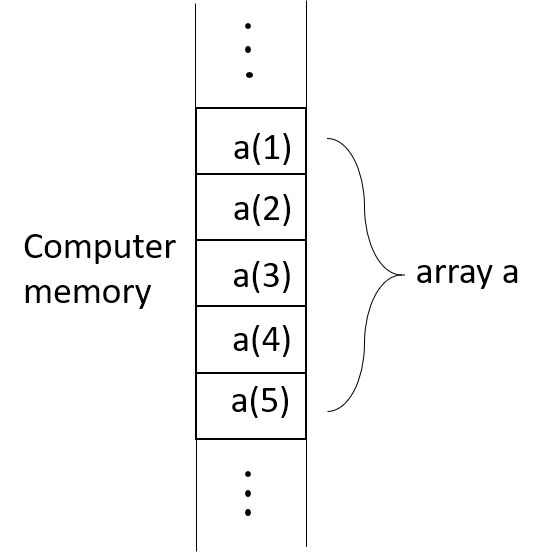
\includegraphics[scale=.75]{Picture1.png}
        \caption{The elements of an array occupy successive locations in a computer memory}
        \label{fig:array}
    \end{figure}
    For example, the first variable shown in figure \ref{fig:array} is referred as a(1). The subscript of an array is of type \code{integer}. Either constants or variables may be used for array subscripts. Arrays can be extremely powerful tools for manipulating data in Fortran. They permit us to apply the same algorithm over and over again to many different data items with simple \code{do} loops. It is possible to manipulate and perform calculations with individual elements of arrays one by one, with whole arrays at once, or with various subsets of arrays.\\

    Mathematically, we often denote the whole array by its subscripted name. e.g., x for $ \{x_i\} $ or a for $ \{a_{ij}\} $. Whist subscripted variables are important in any programming languages, it is the ability to refer to ah array as a whole, without subscripts, which makes Fortran particularly valuable in engineering. The ability to refer to just segments of it, e.g., the array section x(4:10) is just like the icing on the cake.
    \section{Some Terminology of Array}
    \subsection{\code{Rank}}
    The number of subscripts declared for a given array is called the \code{rank} of the array.
    \subsection{\code{Dimension}}
    The \code{dimension} attribute in the type declaration statement declares the size of the array .
    \subsection{\code{Size}}
    The \code{size} of an array is the total number of element declared in that array.
    \subsection{\code{Extent}}
    The number of elements in a given dimension of an array is called the \code{extent} of the array in that dimension.
    \subsection{Shape}
    The shape of an array is defined ad the combination of its \code{rank} and the \code{extent} of the array in each \code{dimension}. Thus two arrays have same shape if they have the same \code{rank} and the same \code{extent} in each \code{dimension}.
    \section{Array Declaration}
    Like any other variable arrays need to be declared at the start of a program unit and memory space assigned to them.

    However, unlike scalar variables, array declarations requrire both a type (\code{integer, real, complex, character, logical} or derived type) and a \code{size} or \code{dimension} (number of elements). For e.g.,
    \begin{lstlisting}[numbers=none,escapechar=\%]
        real x(100), y(100)
        %or using dimension attribute%
        real, dimension(100) :: x, y
    \end{lstlisting}
    We might need to change array size consistently in many places, it is safer practice to declare array size as a single parameter. e.g.,
    \begin{lstlisting}[numbers=none]
        integer, parameter :: maxsize = 100
        real x(maxsize), y(maxsize)
    \end{lstlisting}
    By default, the first element of an array has subscript 1. It is possible to make the array start from subscript zero (or any other positive or negative integer) by declaring the lower bound as well. For example, to start at zero instead of one,
    \begin{lstlisting}[numbers=none]
        real x(0:99)
    \end{lstlisting}
    \section{Dynamic Arrays}
    An obvious problem arises, what if the number of points n is greater that the declared size of the array (here, 100)?

    One not-very-satisfactory solution is to check for adequate space, prompting the user to recompile if necessary with a larger array size.
    \begin{lstlisting}[numbers=none]
        read (10,*) n
        if (n > maxsize) then
            print*, "Sorry, n>maxsize. Please recompile with larger array"
            stop
        end if
    \end{lstlisting}
    A far better solution is to use dynamic memory allocation; that is, the array size is determined (and computer memory allocated) at run-time, not in advance during compilation. To do this one must use \code{allocatable} arrays as follows\begin{enumerate}
        \item In the array declaration statement, use the \code{allocatable} attribute, e.g.,
        \item \begin{lstlisting}[numbers=none]
            real, allocatable :: x(:), y(:)
        \end{lstlisting}
        Note that the shape, but not size is indicated at compile time by a single colon (:).
        \item Once the size of the array has been identified at run-time, allocate them the required amount of memory:
        \begin{lstlisting}[numbers=none]
            read (10,*) n
            allocate (x(n), y(n))
        \end{lstlisting}
        \item When the arrays are no longer needed recover memory by deallocating them:
        \begin{lstlisting}[numbers=none]
            deallocate (x, y)
        \end{lstlisting}
    \end{enumerate}
    \section{Elemental Operations}
    Some times we want to do something to every element of an array.\\The expression \code{x * x} is a new array with elements $ \{{x_i}^2\} $.\\
    The expression \code{sum (x * x)} therefore produces $ \sum {x_i}^2 $\\
    Using many of these features a shorter version of the above program is given bellow
    \lstinputlisting{regressionElemental.f90}
    \section{Matrices and Higher-Dimension Arrays}
    A m$ \times $n arrays of number of the form $ \begin{pmatrix}
            a_11 &\dots & a_1n\\
            \vdots & \ddots & \vdots\\
            a_m1 & \dots & a_mn
        \end{pmatrix} $ is called a matrix (or rank-2 array). The typical element if denoted by $ a_ij $. It has two subscripts. Fortran allows matrices and infact, arrays of upto 7 dimension. In Fortran, the declaration and use of a real $ 3\times 3 $ matrix might look like\begin{lstlisting}[numbers=none]
            real A(3,3)
            A(1,1) = 1.0; A(1,2) = 2.0
            A(1,3) = 3.0; A(2,1) = 4.0    etc
        \end{lstlisting}
    \section{Matrix Multiplication} Suppose A, B and C are $ 3\times3 $ matrices declared by\begin{lstlisting}[numbers=none]
        real dimension (3,3) :: A, B, C
    \end{lstlisting} 
    The statement \code{C=A*B} does element-by-element multiplication; each element C is the product of the corresponding elements in A and B.

    To do "proper" matrix multiplication use the standard \code{matmul} function: \begin{lstlisting}[numbers=none]
        C = matmul(A, B)
    \end{lstlisting}
    A similarly use =ful function is that computing the transpose of a matrix :
    \begin{lstlisting}[numbers=none]
        C = transpose (A)
    \end{lstlisting}
    \section{Array Constants} Array constants may also be defined. An array constant is an array consisting entirely of constants. It is defined by placing the constant values between special delimiters, called array constructors. The starting delimiter of a Fortran array constructor is \code{(/} (old) or \code{[} (modern) and the ending delimiter of an array constructor is \code{/)} or \code{]}. e.g., \code{(/ 1, 2, 3, 4 /)} or \code{[ 1, 2, 3, 4 ]}
    \part{Assignment}
    \begin{enumerate}
        \item Write a program that prompts the user for a positive integer N and output to the screen the partial sum
        \[S_N=\frac{1}{2^2}+\frac{2}{3^2}+\frac{3}{4^2}+\dots+\frac{N}{(N+1)^2}\]
        Find the output of your program for N=20
        \item Write a program to evaluate the binomial coefficient
         \[\binom{n}{r}=\frac{n!}{r!(n-r)!}\] for non-negative integer values of n and r input by the user.\\
        Use your program to evaluate the binomial coefficients $\displaystyle \binom{6}{4},\binom{50}{0},\binom{50}{50},\binom{40}{4},\binom{40}{36} $ 
        \item Write a program that will for any positive integer N input by the user, output the Fibonacci sequence 1,1,2,3,5,\dots up to, but not exceeding N.
    \end{enumerate}
    \part{Lab}
    \begin{itemize}
        \item Example of \code{if} statements\lstinputlisting[caption=Mark to Grade convert using if statement]{lab1.f90}\newpage
        \item Example of \code{select case} statements\lstinputlisting[caption=Mark to Grade convert using select case statement]{lab2.f90}\newpage
        \item Consider the following program to fit a straight line to the set of points $ (x_1, y_1), (x_2, y_2),\dots,(x_n, y_n) $ and then print them out with the best-fit straight line. The data file assumed to be of the form shown bellow 
        \begin{verbatim}
            -------------
            | n         |
            | x1  y1    |
            | x2  y2    |
            | ... ...   |
            | xn  yn    |
            -------------
        \end{verbatim}
        and the best-fit straight line is $ y=mx+c $ where,
        $$ m=\frac{\frac{\sum xy}{n}-\bar{x}\bar{y}}{\frac{\sum x^2}{n}-\bar{x}^2},\, c=\bar{y}-m\bar{x}, \text{ where } \bar{x}=\frac{\sum x}{n},\, \bar{y}=\frac{\sum y}{n}$$
        \lstinputlisting[caption=Example of array using best-fit line problem]{regression.f90}
        \item l
        \item l
    \end{itemize}
    
    
    
    \part{Questions from Past Years}
    % \section{2012}
    % \begin{enumerate}
    %     \item \begin{enumerate}
    %         \item (2 marks) Write down the rules for naming the variables.
    %         \item (6 marks) Briefly discuss by writing the general form of Type Specification statements, Implicit statement and what is the default rule for undeclared variables.
    %         \item (4 marks) Write FORTRAN equivalent's against each of the following mathematical expressions: 
    %         \begin{enumerate}
    %             \item $ \log_e\left|\sec x + \tan x\right|+e^{mx}+\sin(ax+b) $
    %             \item $ a\frac{b}{c}+\log_{10}\left(\cos (xy)\right)+\sqrt{k-bc} $
    %             \item $ x^{2m}+y^x+a^b \ln\left(a+\abs{b}\right)+\sinh(x^2+2) $
    %             \item $ \frac{e^{x+y+2}}{\sin(x+1)+\cos(x+y)}+\frac{ab}{c-d^2}+\frac{ba}{a+\frac{c}{\abs{d}}} $
    %         \end{enumerate}
    %     \end{enumerate}
    %     \item \begin{enumerate}
    %         \item (4 marks) What are the logical statements that are used to code all the computer processing?
    %         \item (4 marks) What is the purpose of using assignment statement? Write down the general form of an assignment statement. Suppose the values of a and b are 10 and 20 respectively. Find the output if the following program is executed: 
    %         \begin{lstlisting}[numbers=none]
    %             integer a,b,c
    %             read* a,b
    %             c=a
    %             a=b
    %             b=c
    %             print*, a,b,c
    %         \end{lstlisting}
    %         \item (6 marks) Which of the following are not acceptable as assignment statements and why?\\ \begin{enumerate*}[label={\roman*)},font={\bfseries}]
    %             \item 2=I,
    %             \item I=J+2,
    %             \item A='2'+'3',
    %             \item A*B*C=D*E*F.
    %             \end{enumerate*}
    %     \end{enumerate}
    %     \item \begin{enumerate}
    %         \item (4 marks) Assume that at the beginning of each of the following program fragment NRD=5 and JOC=8, NDD=?
    %         \begin{enumerate}
    %             \item \begin{lstlisting}
    %                 IF(2*NRD.EQ.JOC)NRD=NRD+2
    %                 NRD=NRD+3
    %             \end{lstlisting}
    %         \end{enumerate}
    %     \end{enumerate}
    %     \item a
    %     \item a
    %     \item a
    %     \item a
    %     \item a
    %     \item a
    %     \item a
    % \end{enumerate}
    \section{2019}
    \begin{enumerate}
        \item \begin{enumerate}
            \item (2 marks) Briefly explain various types of constants used in FORTRAN.
            \item (4 marks) What do you mean by variable in FORTRAN? Write the rules for naming a variable in FORTRAN. Explain which of the variables names in FORTRAN are valid or invalid and why?\\
            \begin{enumerate*}[label={\roman*)},font={\bfseries}]
                            \item Mathematics
                            \item STOP
                            \item ORPS
                            \item width
                            \end{enumerate*}
            \item (2 marks) How is the type of a variable in FORTRAN specified? Explain with example.
            \item (4 marks) Write the FORTRAN expressions for each of the following mathematical expressions:\\
            \begin{enumerate}
                \item $ \abs{\sqrt{a-b^2}-\frac{c^2}{a/b}} $
                \item $ \cos(2x-y)+\abs{x^2+y^2}+e^{xy} $
                \item $ \cos^{-1} x+\tan x^2+e^{mx}+x^3y^2e^{\abs{x}}  $
                \item $ (a^n)^m+a^na^m+\ln(a+bx^2) $
            \end{enumerate}
        \end{enumerate}
        \item \begin{enumerate}
            \item (2 marks) The following IF construct is incorrect, why? Also write the correct form with flow chart.
            \begin{lstlisting}[numbers=none]
                IF (x<y)c=a+b*d
                    ELSE IF (x==y) c=d
                    a=b
                    ELSE IF (x>y) THEN c=a-b/e+f
                    ELSE e==f+g
                        ENDIF
            \end{lstlisting}
            \item (6 marks) Write the appropriate subprogram and main program to\\
            \begin{enumerate*}[label={\roman*)},font={\bfseries}]
                \item interchange two values
                \item sort an ascending array A(1),A(2),\dots,A(N) to a descending array using the subprogram in (i)
            \end{enumerate*} 
            \item (4 marks) THe commission on a clerk's total SALES is as follows:
            \begin{enumerate}
                \item IF SALES<\$50, then there is no commission
                \item IF \$50$ \leq $ SALES $ \leq $ \$250, then commission =10\% of SALES
                \item IF SALES>\$250, then commission =\$20+8\% of SALES above \$250
            \end{enumerate}
        \end{enumerate}
        \item \begin{enumerate}
            \item (4 marks) What do you mean by a DO loop? Write the general form of DO statement and explain its functionality. What is the terminal statement of a DO loop?
            \item (2 marks) Find the final value of K after the following FORTRAN program segment is executed:
            \begin{lstlisting}[numbers=none]
                    K=2
                10 DO 20 I+3,8,2
                IF (1 .EQ. 5) GO TO 20
                    K=K+1
                  20 CONTINUE
                    k=2*k
            \end{lstlisting}
            \item (6 marks) Write an algorithm, draw flow chart and write the FORTRAN program that reads an integer N and prints the sum of the series: $ 1^3+2^3+3^3+\dots+N^3 $
        \end{enumerate}
        \item \begin{enumerate}
            \item (6 marks) Write a FORTRAN program to sum the following series using FOR loop and WHILE loop severally $ (1+\frac{1}{2})(1+\frac{1}{2}+\frac{1}{3})\dots(1+\frac{1}{2}+\frac{1}{3}+\dots+\frac{1}{N}) $
            \item (4 marks) If M=12345, N=56789, A=456.123 and B=678.999, find the output after the following statements:
            \begin{enumerate}
                \item \begin{lstlisting}[numbers=none]
                    print 10 M,N,A,B
                    10 format (3x,18x2x17,2x,x(F8.3,2x))
                \end{lstlisting}
                \item \begin{lstlisting}[numbers=none]
                    print 20 A,B,M,N
                    20 format ('1', E12.2||1x,E12.2||1x,218)
                \end{lstlisting}
                
            \end{enumerate}
            \item (2 marks) Locate errors (if any) and correct them:
            \begin{enumerate}
                \item \begin{lstlisting}[numbers=none]
                    read (5,10) A,K,M,Z
                    10 format (F8.0,2x,2318)
                \end{lstlisting}
                \item \begin{lstlisting}[numbers=none]
                    write (6,12) A,B,M
                    12 format (2x,F8.2,2x,I8,x,F8.3)
                \end{lstlisting}
            \end{enumerate}
        \end{enumerate}
        \item \begin{enumerate}
            \item (5 marks) Define an array, dimension statement and parameter statement in FORTRAN. Find the number of elements in the array: DIMENSION P(1:10), T(2:5,1:4),S(0:3,2:5,3:4)
            \item (2 marks) Which of the following array names in FORTRAN are valid or invalid and why?\\
            \begin{enumerate*}[label={\roman*)},font={\bfseries}]
                            \item xx(3*4,6);
                            \item XY(N+3,M);
                            \item YZ(A,L,P);
                            \item ZX(1=1+1)
                            \end{enumerate*}
            \item (5 marks) Four test are given to a class of 10 students. Write a program that calculates the average score of each student and the average score in each test.
        \end{enumerate}
        \item \begin{enumerate}
            \item (3 marks) What do you mean by main program and subprogram? What are the main differences between a function subprogram and a subroutine subprogram?
            \item (5 marks) What is meant by format directed input  and output? Explain the I-format, F-format, E-format and A-format specification statement in FORTRAN.
            \item (5 marks) Briefly explain the file processing in FORTRAN. Explain open fine and close file in FORTRAN.
        \end{enumerate}
    \end{enumerate}
\end{document}